\section{项目功能设计}

\subsection{大雾实验工具}

\subsubsection{总体功能说明}

本工具通过腾讯云服务器搭建于网页平台,支持任何设备自由访问。
传入实验数据后,本工具立刻完成绘制图像、计算不确定度、生成计算公式等一系列操作,
并将最终结果整理成一份 Word 文档,下载后即可直接使用。
本实验工具支持一级大物的 25 个实验,如图 \ref{fig:main} 所示,这大大提升了学生们撰写实验报告的效率。
由于本工具只是将传入的实验数据进行自动分析,故其不会造成抄袭、造假等学术不端问题。

\begin{figure}[p]
  \centering
  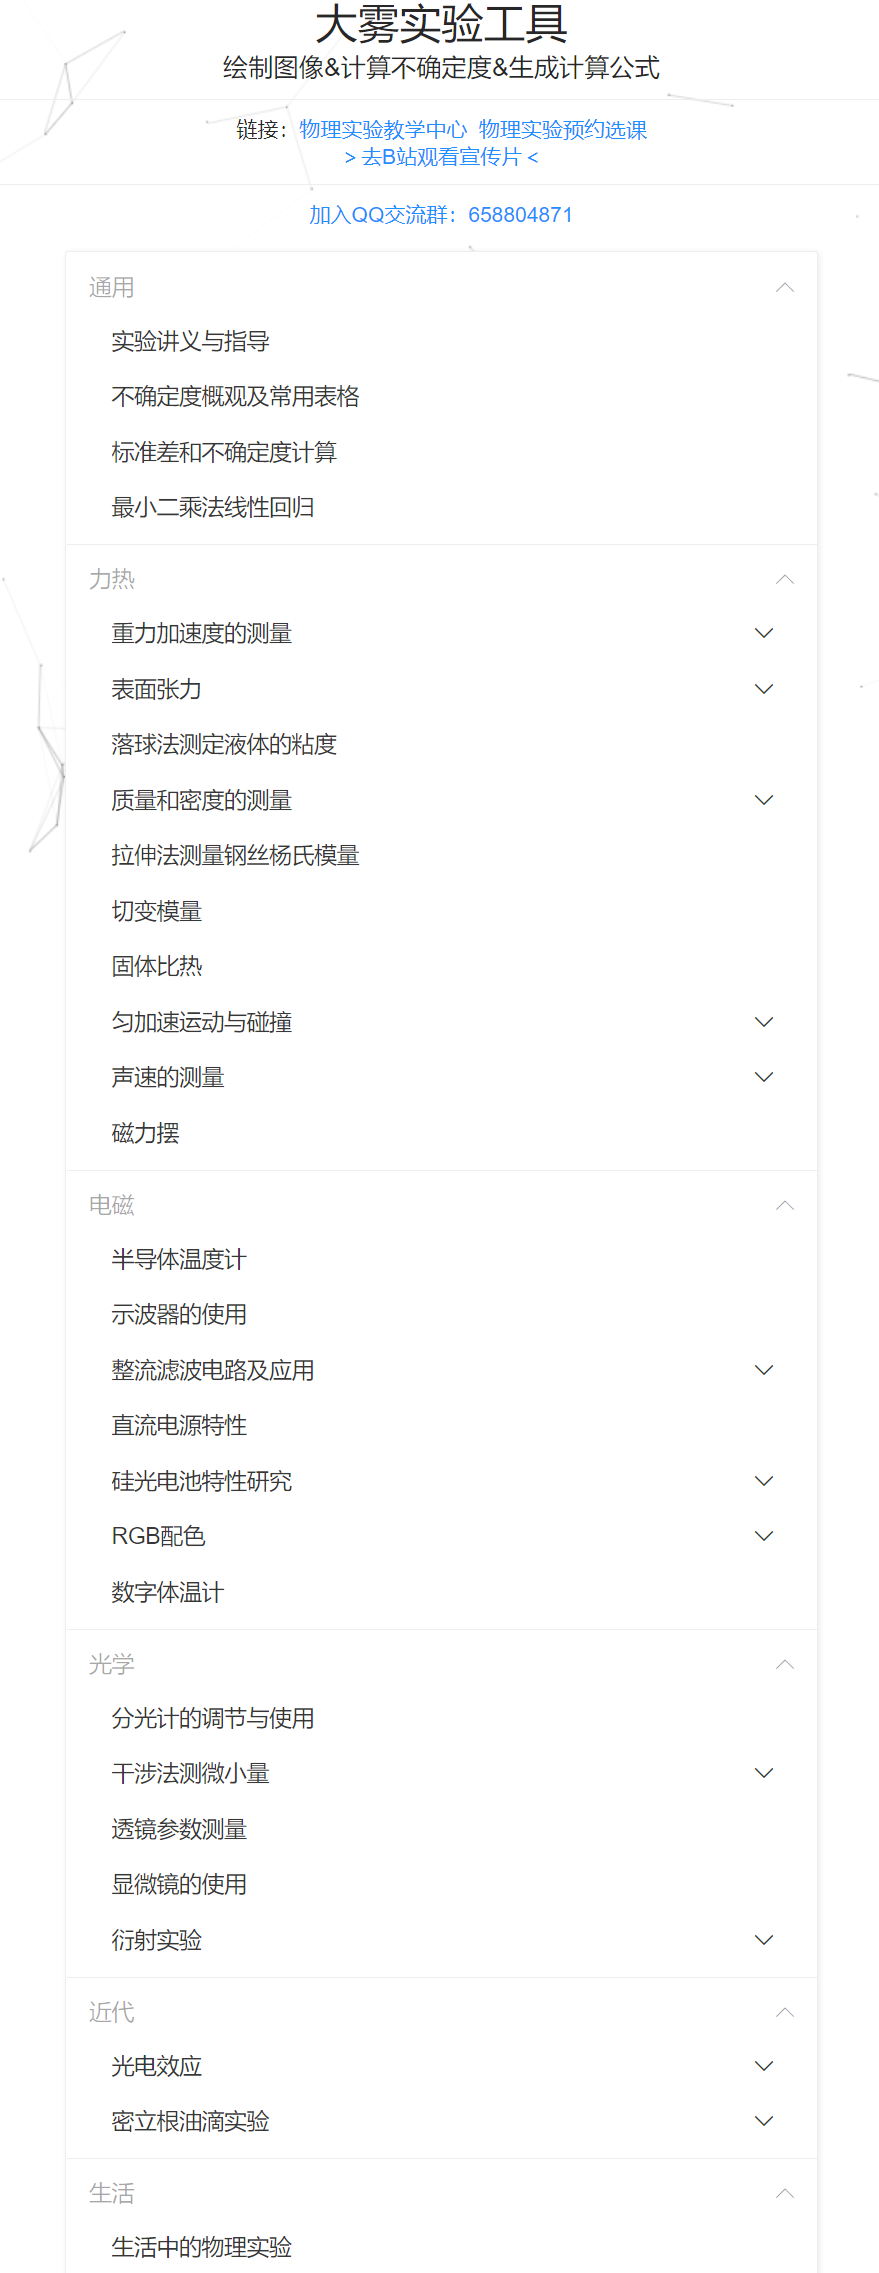
\includegraphics[height=0.95\textheight]{figure/main.png}
  \caption{大雾实验工具网站主界面}
  \label{fig:main}
\end{figure}

\subsubsection{具体功能点说明}

使用本工具时,用户只需输入他们做实验时测量到的原始数据,
而无需任何额外的计算处理,用户所要做的只有按照规定的格式上传 Excel 文档。
本工具支持 \verb|xlsx|, \verb|csv| 等各种格式的数据表格。
具体而言,每个实验都会有一张示例数据表供用户参考,如图 \ref{fig:interface} 的界面所示。
用户也可以直接下载示例数据,并直接在它的基础上进行修改。
因此,本工具没有任何学习成本,是一款即点即用、免安装的简单轻应用。

\begin{figure}[p]
  \centering
  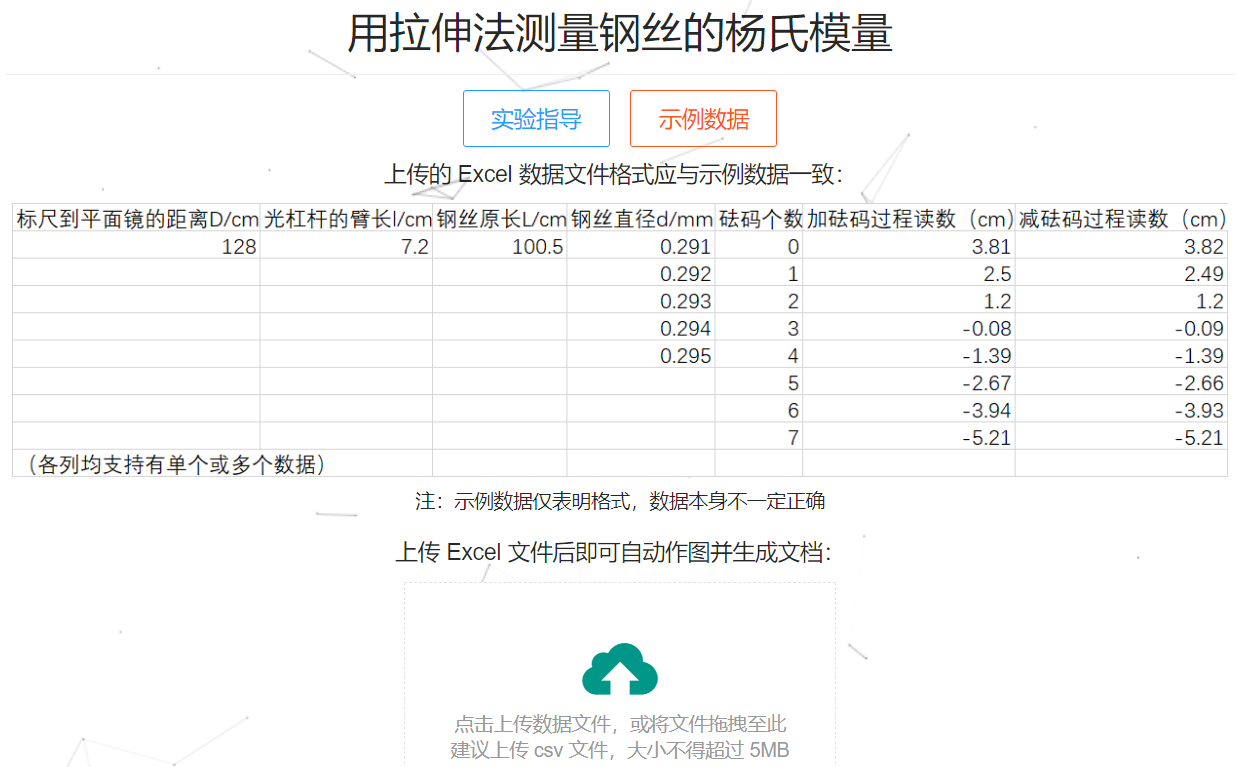
\includegraphics[width=0.67\columnwidth]{figure/interface.png}
  \caption{“拉伸法测钢丝杨氏模量”的工具界面}
  \label{fig:interface}
\end{figure}

另外,本工具贴心地提供了不确定度表格与通用的计算工具,并且每个实验都附有可在线浏览的实验指导。

{\noindent\bfseries\textbullet{}绘制图像}

本工具根据输入的数据以及实验原理,自动生成美观的实验图像,
支持平滑去噪、数据拟合、双 y 图等多种图像生成需求,如图 \ref{fig:draw} 所示。

\begin{figure}[p]
  \centering
  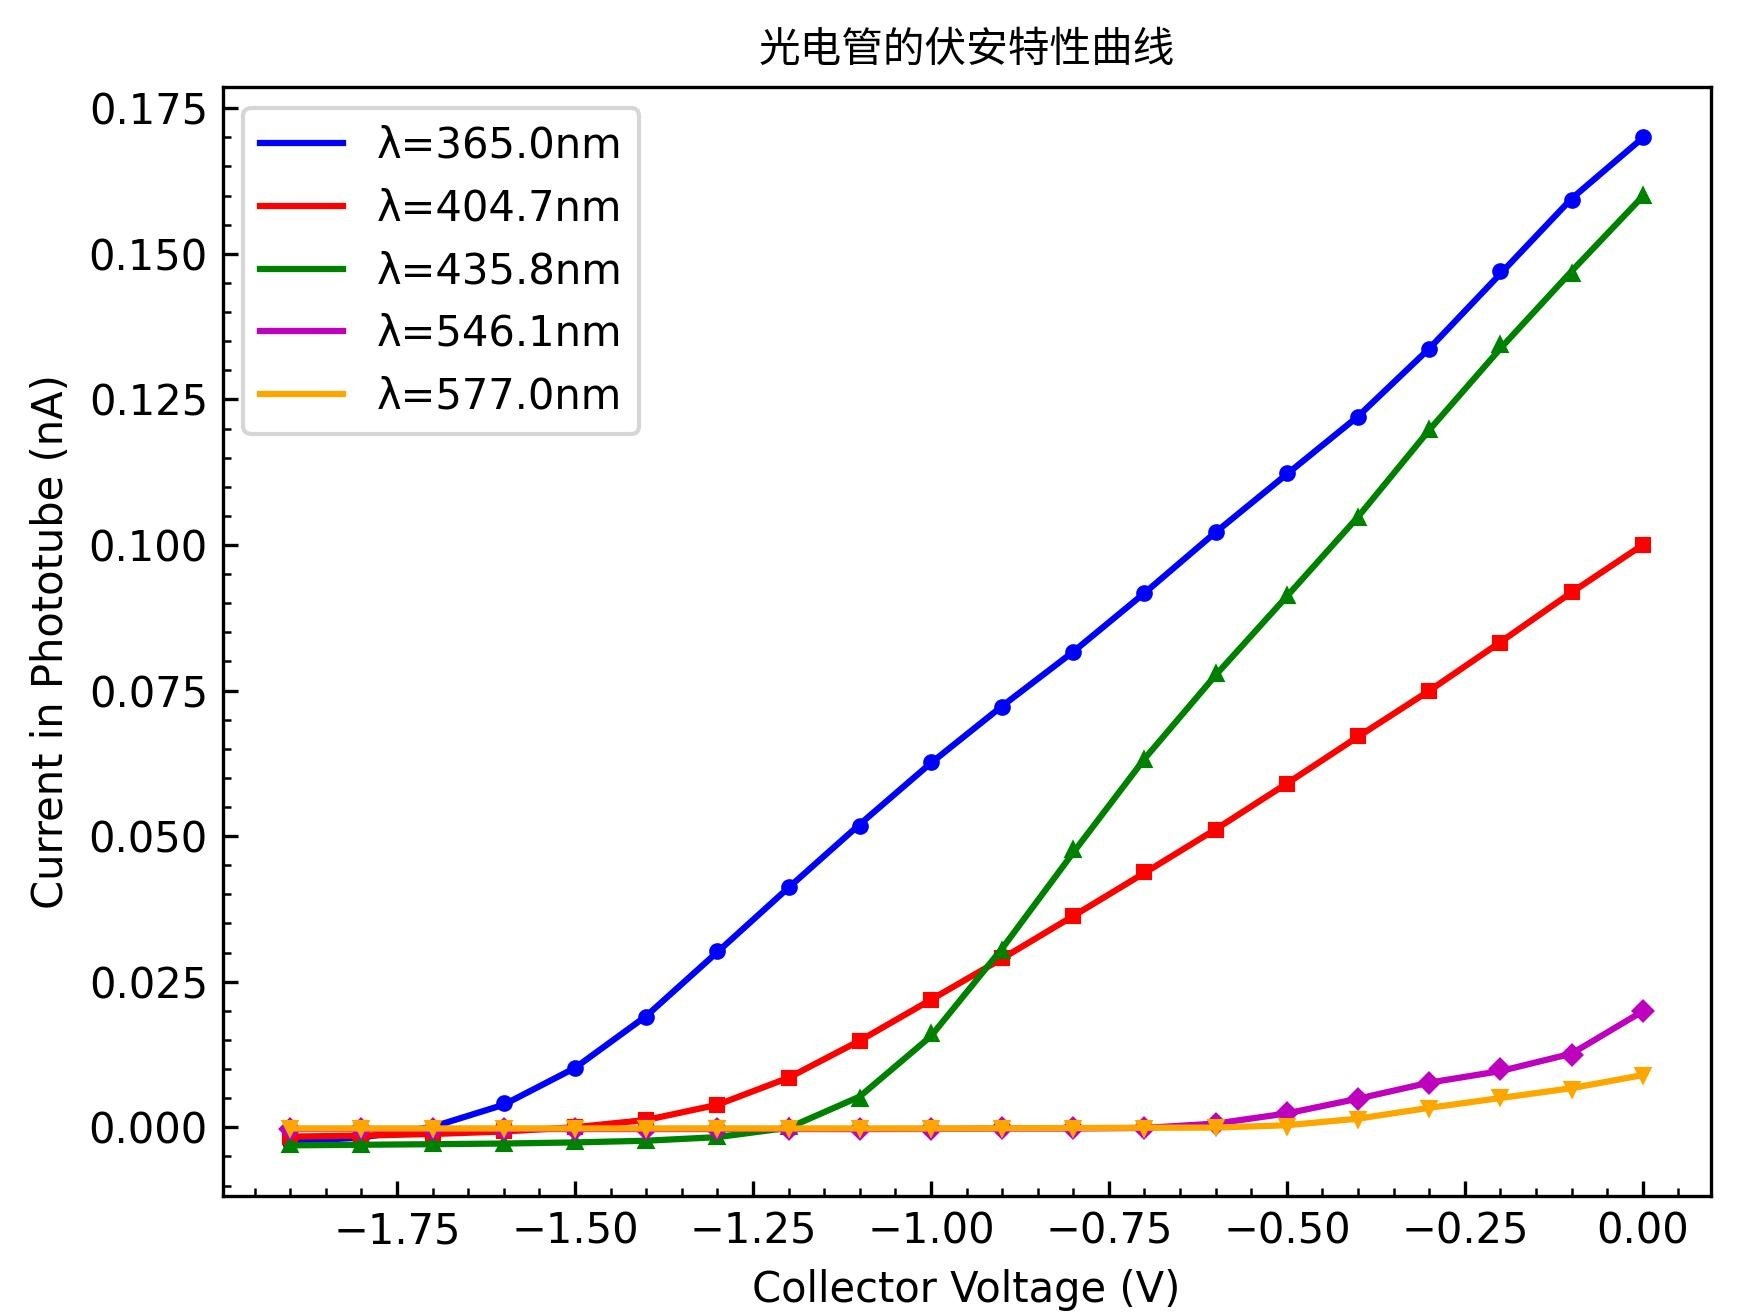
\includegraphics[width=0.67\columnwidth]{figure/draw.jpg}
  \caption{平滑连接的光电效应伏安特性曲线}
  \label{fig:draw}
\end{figure}

{\noindent\bfseries\textbullet{}计算不确定度与生成计算公式}

本工具在生成的 Word 文档中渲染了各种公式,如图 \ref{fig:calc} 所示。
用户可以直观看到不确定度每一步的计算过程,并在自己的报告中直接使用这些算式与结果。

\begin{figure}[p]
  \centering
  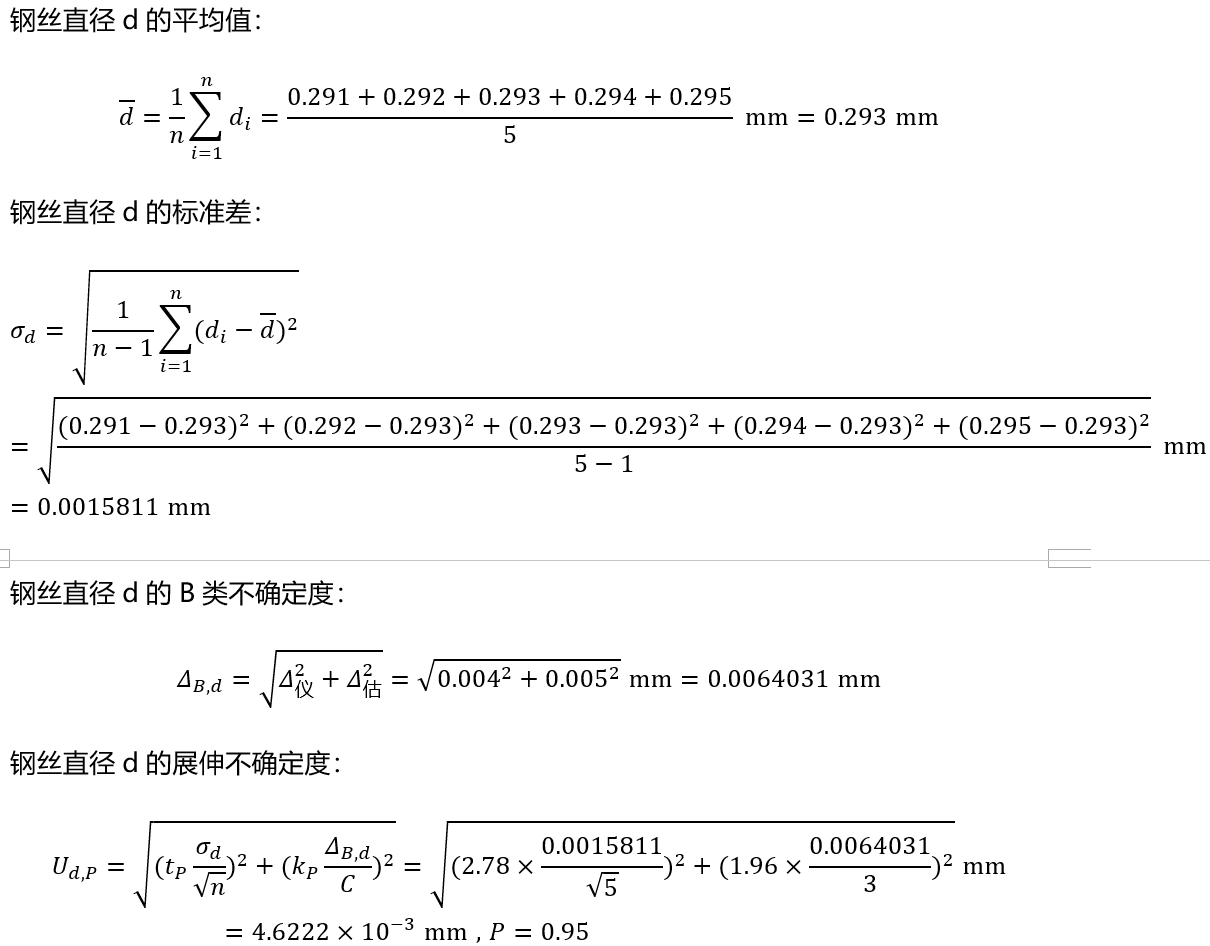
\includegraphics[width=0.67\columnwidth]{figure/calc.png}
  \caption{不确定度计算的详细过程}
  \label{fig:calc}
\end{figure}

在 Word 文档中除了有已经渲染好的公式外,
我们还提供了它们的 \LaTeX{} 源码,如图 \ref{fig:latex} 所示。
这极大方便了用 \LaTeX{}, Markdown 等排版实验报告的用户,使他们无需手动敲入每一个算式。

\begin{figure}[htbp]
  \centering
  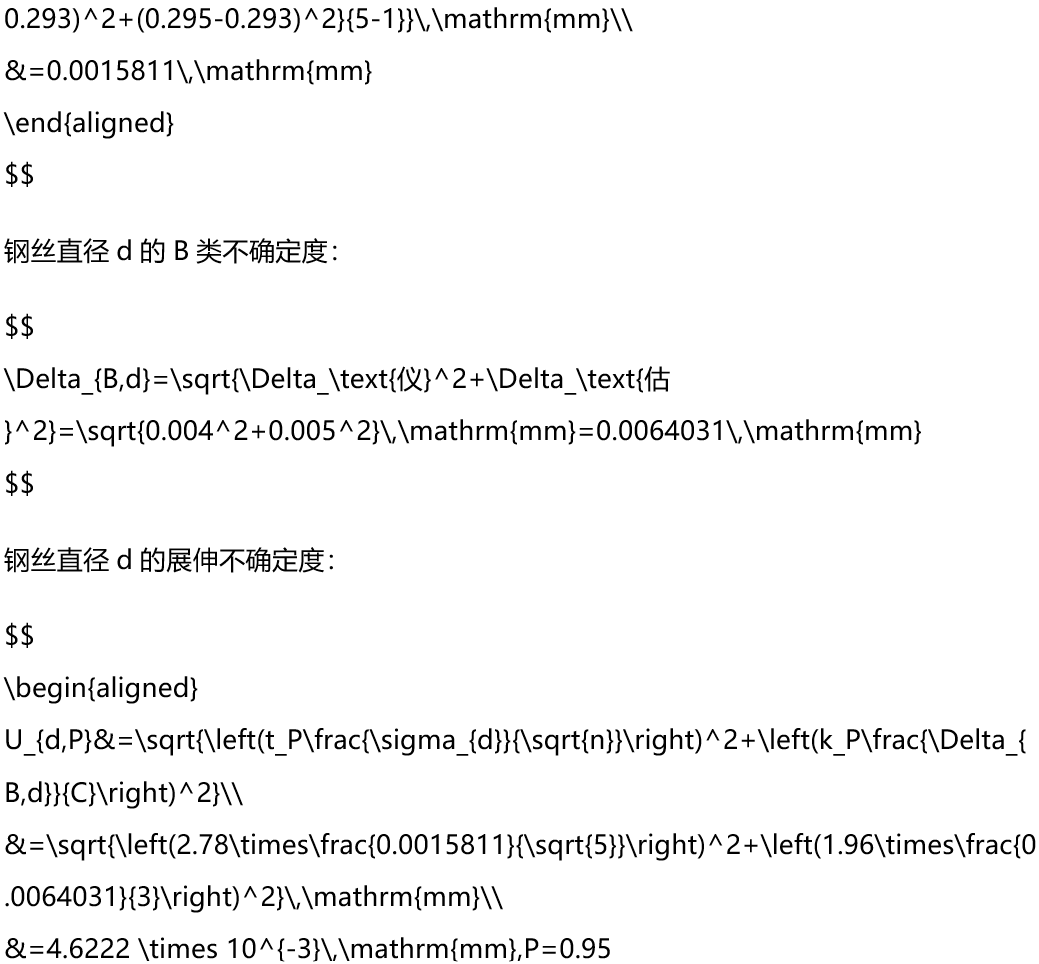
\includegraphics[width=0.67\columnwidth]{figure/latex.png}
  \caption{不确定度算式的 \LaTeX{} 源码}
  \label{fig:latex}
\end{figure}

\subsubsection{功能点设计细节}

本工具后端使用 Python 编写,使用的包与模块如表 \ref{tab:pkg} 所示。
前端由 HTML 编写,并使用了 \verb|Flask| Web 应用框架。以下将详细介绍各功能的实现,分为图像绘制、数据处理和文档生成三部分。

\begin{table}[htbp]
  \caption{本工具使用的全部 Python 包与模块}
  \label{tab:pkg}
  \vskip 0.1in
  \centering\small
  \begin{tabular}{lc}
  \toprule
  Python 包或模块 & 用途 \\
  \midrule
  \verb|chardet| & 检测用户上传的数据表格的编码 \\
  \verb|collections| & 通过 \verb|namedtuple| 使代码更清晰 \\
  \verb|Flask| & Web 应用框架 \\
  \verb|latex2mathml| & \LaTeX{} 代码转换为 \verb|MathML| 代码 \\
  \verb|lxml| & \verb|MathML| 代码转 \verb|Office MathML| \\
  \verb|math|, \verb|numpy| & 不确定度数字运算 \\
  \verb|Matplotlib| & 绘制物理图像 \\
  \verb|os|, \verb|random|, \verb|shutil| & 后台文件操作与管理 \\
  \verb|pandas| & 数据表格处理 \\
  \verb|python-docx| & 生成 Word 文档 \\
  \verb|SciPy| & 数据拟合 \\
  \verb|SymPy| & 不确定度符号运算 \\
  \verb|time|, \verb|threading| & 定时删除生成的 Word 文档 \\
  \verb|traceback| & 打印运行错误以便调试 \\
  \bottomrule
  \end{tabular}
  \vskip -0.1in
\end{table}

\subsubsection{图像绘制}

图像由 \verb|Matplotlib| 绘制。我们的规范如下:
\begin{itemize}
  \item 面向绘图对象作图:\verb|fig, ax = matplotlib|\\\verb|.pyplot.subplots()|
  \item 设置副刻度为主刻度的一半,主刻度为默认:\verb|ax.xaxis.set_minor_locator(matplotlib|\\\verb|.ticker.AutoMinorLocator(2))|
  \item 刻度朝内:\verb|matplotlib.rcParams["xtick|\\\verb|.direction"] = matplotlib.rcParams|\\\verb|["ytick.direction"] = "in"|
  \item 若一张图有且只有一组点线,则点使用红色(\verb|color="r"|),线使用蓝色(\verb|color="b"|),且线覆盖在点的上面;若一张图有多组点线,则同一组点线的颜色应当相同,并依次使用蓝(\verb|b|)、红(\verb|r|)、绿(\verb|g|)、紫(\verb|m|)、橙(\verb|orange|)、青(\verb|c|)。
  \item 点的类型使用实心圆(\verb|"o"|),若一张图有多组点线,则依次使用实心圆(\verb|o|)、正方形(\verb|s|)、上三角(\verb|^|)、菱形(\verb|D|)、下三角(\verb|v|)、星号(\verb|*|)。
  \item 线条粗细使用 \verb|linewidth=1.5|, 点的大小使用 \verb|markersize=3|, 可视数据量、数据组数适当调整,但应保持统一性。
  \item 绘制双 y 轴图使用 \verb|matplotlib.axes.Axes| 对象的 \verb|twinx()| 方法。
  \item 只有一组点线的图,一般不显示图例。
  \item 图像字体:\verb|SourceHanSansSC-Regular.otf|
  \item 轴标签和标题中的物理量名称与单位应使用 \LaTeX{}。
\end{itemize}

\subsubsection{数据处理}

无论使绘制图像时的线性拟合,还是计算不确定度的大小,都绕不开数据处理。
我们利用 \verb|pandas|, \verb|SciPy|, \verb|SymPy| 等包自主编写了 \verb|calc.py| 应用程序接口,
它提供以下函数:
\begin{description}
  \item[科学计数法输出] \verb|numlatex: (num: float,|\\\verb|prec: int = 5) -> str|\\
  \fbox{返回一个数的科学计数法形式的 \LaTeX{} 代码}\\
  \verb|num|: 要转成科学计数法的数字\\
  \verb|prec|: 有效数字位数(默认值:5)
  \item[不确定度计算] \verb|analyse: (data: pandas.DataFrame,|\\\verb|delta_b1: float = 0., delta_b2: float|\\\verb|= 0., symbol: str = "x", unit: str = "",|\\\verb|confidence_C: float = 3., confidence_P:|\\\verb|float = 0.95) -> AnalyseData|\\
  \fbox{计算一组数据的平均值、标准差、不确定度}
  \verb|data|: 要处理的一组实验数据\\
  \verb|delta_b1|: 仪器最大允差 \(\Delta_\text{仪}\)(默认值:0)\\
  \verb|delta_b2|: 估读最大允差 \(\Delta_\text{估}\)(默认值:0)\\
  \verb|symbol|: 数据的物理符号(默认值:\verb|"x"|)\\
  \verb|unit|: 数据的单位(默认值:\verb|""|)\\
  \verb|confidence_C|: 置信系数 \(C\)(默认值:3)\\
  \verb|confidence_P|: 置信概率 \(P\)(默认值:0.95)\\
  \verb|AnalyseData|: 数据计算结果的集合
  \item[最小二乘法线性回归] \verb|analyse_lsm: (data_X:|\\\verb|pandas.DataFrame, data_Y: pandas|\\\verb|.DataFrame, symbol_X: str = "X",|\\\verb|symbol_Y: str = "Y", unit_m: str = "",|\\\verb|unit_b: str = "") -> AnalyseLsmData|\\
  \fbox{将一组数据用最小二乘法拟合成一条直线}\\
  \verb|data_X|: x轴数据(自变量数据)\\
  \verb|data_Y|: y轴数据(因变量数据)\\
  \verb|symbol_X|: 自变量物理符号(默认值:\verb|"X"|)\\
  \verb|symbol_Y|: 因变量物理符号(默认值:\verb|"Y"|)\\
  \verb|unit_m|: 斜率的单位(默认值:\verb|""|)\\
  \verb|unit_b|: 截距的单位(默认值:\verb|""|)\\
  \verb|AnalyseLsmData|: 直线拟合结果的集合
  \item[不确定度合成] \verb|analyse_com: (exp: str, varr:|\\\verb|tuple = (), constt: tuple = (), unit:|\\\verb|str = "", confidence_P: float = 0.95)|\\\verb|-> AnalyseComData|\\
  \fbox{根据表达式计算物理量的值和不确定度}\\
  \verb|exp|: 物理量计算表达式(字符串),为一个物理量=一些物理量(或常量)之积与之商的形式,如 \verb|E=4*pi**2*l/T**2| 代表 \(E=\frac{4\pi^2l}{T^2}\)\\
  \verb|varr|: 物理量(元组),元组的每个元素均为元组,该子元组的第 1 个元素为物理量名,第 2 个元素为物理量值,第 3 个元素为其不确定度(默认值:\verb|()|)\\
  \verb|constt|: 常量(元组),元组的每个元素均为元组,该子元组的第 1 个元素为常量名,第 2 个元素为常量值(默认值:\verb|()|)\\
  \verb|unit|: 要计算的物理量的单位(默认值:\verb|""|)\\
  \verb|confidence_P|: 置信概率 \(P\)(默认值:0.95)\\
  \verb|AnalyseComData|: 不确定度合成结果的集合
\end{description}

\subsubsection{文档生成}

Word 文档由 \verb|python-docx| 生成。我们的规范如下:
\begin{itemize}
  \item 字体使用微软雅黑:\verb|document.styles|\\\verb|['Normal'].font.name = "微软雅黑"|
  \item 文档第一行是实验名称:\\\verb|document.add_paragraph(name())|\\随后注明:\\“【Latex 代码在下面,请向下翻阅】”
  \item 内容跨度较大的段落之间应当用一个空行。
  \item 文档中插入的数据一般保留 4 或 5 位有效数字:\verb|"%.5g"%x|, 线性拟合的相关系数 \(r\) 保留 8 位有效数字。
  \item 若某张图片正好在第 2 页开头,而第 1 页尾部有很多空白区域,为避免误解,应在第1页的最后一个段落之后注明“【本文档不只有一页,请向下翻阅】”。
  \item 插入表格使用 \verb|docx.document.Document| 对象的 \verb|add_table()| 方法。
\end{itemize}

鉴于不确定度的计算方法是固定的、算法化的,我们利用 \verb|lxml| 等包自主编写了 \verb|insert.py| 应用程序接口,
这样只需调用几个函数,就可以在 Word 文档中完成数学算式的渲染与添加。具体可见公式插入 API 的说明文档,这里不再赘述。

\subsection{蜗壳排课工具}

该工具是一个网页应用,使用方便快捷。在主页面,已添加的课程列表会被清晰地展示出来,用户可以通过点击“添加课程”、“编辑课程”或“开始排课”,进入相应的界面,如图 \ref{fig:p1} 所示。

\begin{figure}[htbp]
  \centering
  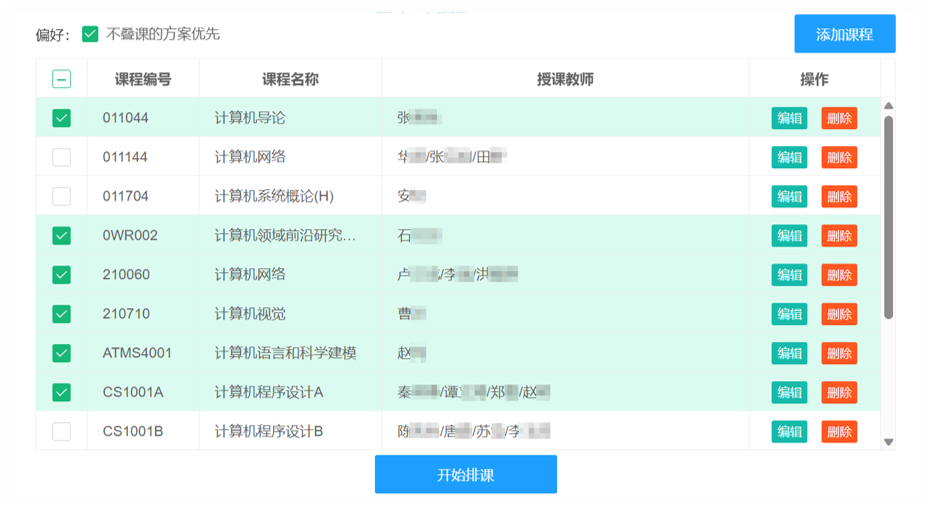
\includegraphics[width=\columnwidth]{figure/p1.png}
  \caption{蜗壳排课工具主页}
  \label{fig:p1}
\end{figure}

图 \ref{fig:p2} 展示了本工具的“添加课程”页面。在此页面,用户可以通过各种信息,如课程编号、课程名称、教师名称等进行课程搜索,我们的网站已经收录了超过 2500 个课程,并会定期从教务系统自动更新。此外,我们还引入了评课社区的课程评级,供用户参考。在添加课程时,用户可以为每个课程设定一个喜好程度,然后工具会根据这个喜好程度和课程时间自动进行课程安排。

\begin{figure}[htbp]
  \centering
  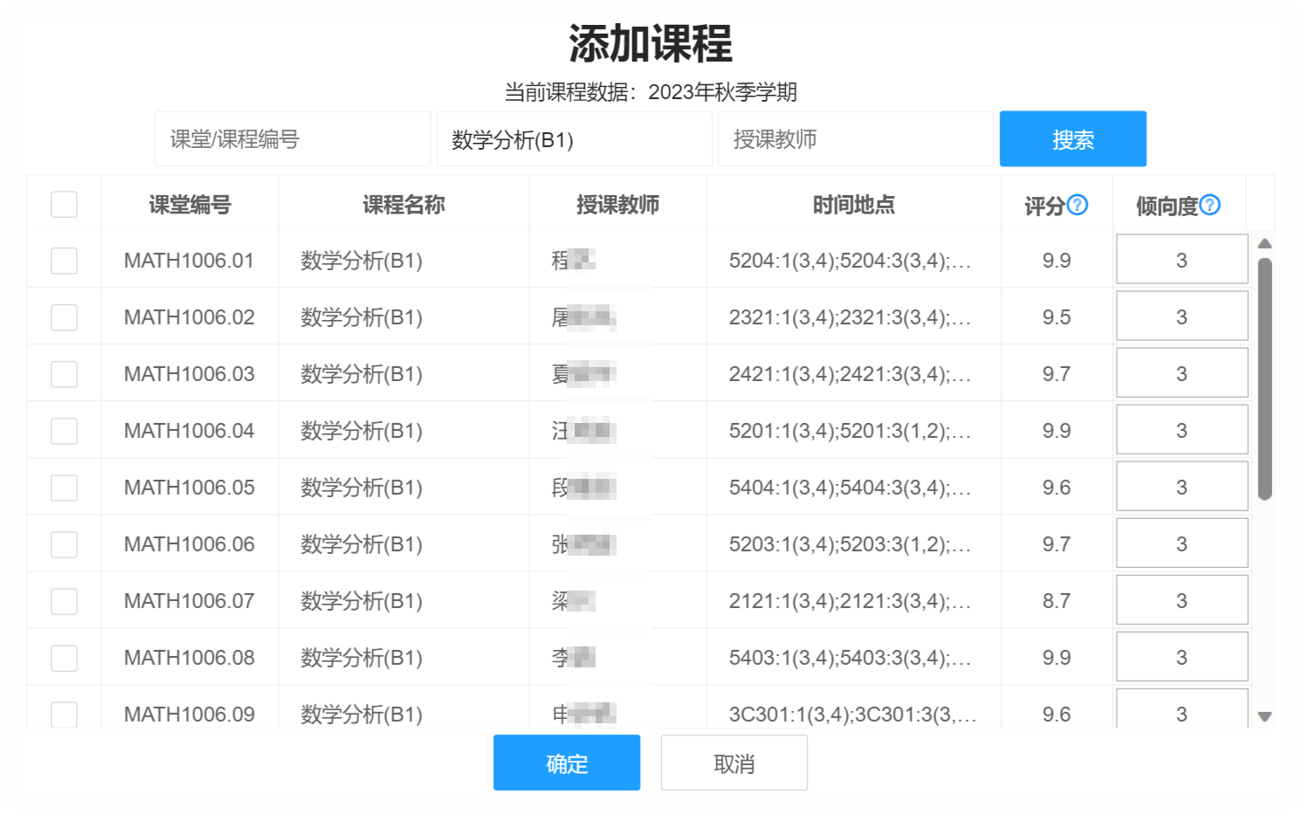
\includegraphics[width=\columnwidth]{figure/p2.png}
  \caption{蜗壳排课工具“添加课程”页面}
  \label{fig:p2}
\end{figure}

我们的工具提供的课程排列方案,既包括明确的列表形式,也包括直观的课程表形式。虽然课程表的样式与教务系统的基本一致,但我们对其样式做了优化,让它看起来更为清楚易懂,同时对小屏幕设备的兼容性也做了提升。

\subsection{我的科大 APP}

我的科大 APP 提供了包括教室查询、学校周边、校园导航等在内的 34 项链接功能,还有任务清单、资料分享等 7 项我们自主研发的功能,如图 \ref{fig:m1} 所示。然而,软件安装包仅有 \qty{2.5}{\mega\byte},安装后体积也仅 \qty{5}{\mega\byte},可以说是小巧却功能全面。

\begin{figure}[htb]
  \centering
  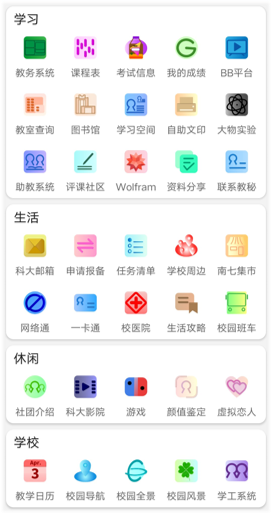
\includegraphics[width=0.8\columnwidth]{figure/m1.png}
  \caption{我的科大 APP 主页}
  \label{fig:m1}
\end{figure}

本项目主要使用 Android Studio 开发工具,结合了 Kotlin 和 HTML, JavaScript, CSS 等多种语言进行开发,可以在 Android 系统上运行。
为了实现统一身份认证和科大邮箱的自动登录,"我的科大"将密码进行加密并保存在本地。这样即使手机中有病毒软件,也难以窃取信息,这就像是一个坚不可摧的防线,万众难以突破。除了为了统计用户量、启动次数、版本分布等收集的去敏化的设备信息,我们并未将任何用户信息上传至服务器。尽管如此,我们还是制定了 APP 的隐私政策,并将严格按照该政策保护用户的信息。
软件已完成了工信部的 ICP 备案并显示备案号。

我们深知,细节决定成败。"我的科大"在图标、文本布局、气泡提示、按钮位置等方面,都遵循了人体工程学的设计原则。我们在用户初次登录邮箱时,为了方便用户,我们预先在邮箱地址中添加了“@mail.ustc.edu.cn”,以防止用户——尤其是新生——遗漏或忘记输入“mail.”。当然,在之后的每次登录中,账号和密码都会自动填写。这些细微的改进,都为用户带来了极致的体验。

我们始终倾听用户的声音。一方面,APP 中设有反馈选项,用户可以通过填写问卷向我们反馈;另一方面,我们还通过用户交流群发布群投票,以不断优化我们的产品。我们采纳了用户的许多有益建议,例如实现了网页内文件下载功能,添加了“科大影院”功能,课程表添加了自定义课程的功能。我们始终将用户体验作为我们的首要任务,不断创新,不断前进。